\documentclass[11pt]{article}

% Page format
\usepackage[margin=1in]{geometry}

% Math packages and custom commands 
\usepackage{framed, tikz}
\usepackage[utf8]{inputenc}
\usepackage{mathtools,amsthm}
\usepackage{enumitem,amssymb}
\usepackage{hyperref}
\definecolor{shadecolor}{gray}{0.9}


\newtheoremstyle{case}{}{}{}{}{}{:}{}{}
\theoremstyle{case}
\newtheorem{case}{Case}
\DeclareMathOperator{\R}{\mathbb{R}}
\DeclareMathOperator{\E}{\mathbb{E}}
\DeclareMathOperator{\Var}{\text{Var}}
\DeclareMathOperator{\Cov}{\text{Cov}}
\newcommand{\bvec}[1]{\mathbf{#1}}
\renewcommand{\P}{\mathbb{P}}
\newcommand{\norm}[2][2]{\| #2\|}
\newcommand{\note}[1]{\noindent{[\textbf{NOTE:} #1]}}
\newcommand{\hint}[1]{\noindent{[\textbf{HINT:} #1]}}
\newcommand{\recall}[1]{\noindent{[\textbf{RECALL:} #1]}}

\DeclareMathOperator*{\argmin}{arg\,min}
\DeclareMathOperator*{\argmax}{arg\,max}


\begin{document}

\begin{center}
{\Large CSCE 790-003, Spring 2022 \\ Assignment 1}

\begin{tabular}{rl}
Username: & [your email username] \\
Name: & [your first and last name] \\
\end{tabular}
\end{center}
By turning in this assignment, I agree by the honor code of USC Columbia.

\paragraph{Submission.}
You need to submit the following files to Blackboard:
\begin{itemize}
    \item A pdf file named as assignment1\_$\langle username \rangle$.pdf, where you replace $\langle username \rangle$ with your email username. This pdf file contains your anwsers to the written problems, including problems 1, 2, 3, and 4(c). 
    You can either edit the assignment1.tex file to fill in your answers and submit the pdf file generated from the edited tex file, or scan and submit your hand-written answers.
    \item A zip file named as assignment1\_$\langle username \rangle$.zip, where you replace $\langle username \rangle$ with your email username. This zip file contains a single file specified in problem 4.
\end{itemize}

\section{Bellman Optimality Operator Is a Contraction [25pt]}
Recall the definition of the Bellman optimality operator $T^*: \mathbb{R}^{|S|} \to \mathbb{R}^{|S|}$, where $|S|$ is the number of states in state space $S$:
\begin{align*}
    (T^*V)(s) := \max_a R(s,a) + \gamma \sum_{s'}P(s'|s,a)V(s')
\end{align*}
for each $s\in S$.
Suppose $\gamma<1$.
Prove that $T^*$ is a $\gamma$-contraction in the infinity norm $\norm{\cdot}_\infty$, i.e. for any $V, V'\in\mathbb{R}^{|S|}$
\begin{align*}
    \norm{T^*V'-T^*V}_\infty\leq\gamma\norm{V'-V}_\infty
\end{align*}
where $\norm{V}_\infty := \max_{s \in S} |V(s)| $.

\underline{Hint:} Since it is the infinity norm, we need to show the inequality holds for each $s\in S$, i.e. $T^*V'(s)-T^*V(s) \leq  \gamma\norm{V'-V}_\infty$.
For any $s\in S$.
Let
\begin{align*}
    a^*_s = \argmax_a R(s,a) + \gamma \sum_{s'}P(s'|s,a)V(s')\\
    a'^*_s = \argmax_a R(s,a) + \gamma \sum_{s'}P(s'|s,a)V'(s')
\end{align*}
be the actions selected by the $T^*$ operator for $V$ and $V'$, respectively.

If $(T^*V')(s) \geq (T^*V)(s)$, try to show that the following holds:
\begin{align*}
    |(T^*V')(s)-(T^*V)(s)|
    =& (T^*V')(s) - (T^*V)(s) \qquad \text{(Since we assumed $(T^*V')(s) \geq (T^*V)(s)$)} \\
    =& R(s,a'^*_s) + \gamma \sum_{s'}P(s'|s,a'^*_s )V'(s') - (R(s, a^*_s) + \gamma \sum_{s'}P(s'|s, a^*_s)V(s')) \\
    \leq& \gamma\norm{V'-V}_\infty
\end{align*}

What if $(T^*V')(s) < (T^*V)(s)$ instead?
\begin{shaded}
Your answer here.
\end{shaded}

\newpage
\section{Performance Difference Lemma and Policy Improvement Theorem [25pt]}
\begin{enumerate}[label=(\alph*)]
\item Let's first prove a useful lemma, called Performance Difference Lemma: For any policies $\pi, \pi'$, and any state $s\in S$,
\begin{align*}
    V^{\pi'}(s) - V^{\pi}(s) = \E_{s'\sim d^{\pi'}_s}[A^\pi(s',\pi')]
\end{align*}
where $d^{\pi'}_s$ is the discounted occupancy induced by policy $\pi'$ by starting from state $s$, i.e.
\begin{align*}
    d^{\pi'}_s(s') = \sum_{t=0}^\infty \gamma^t\Pr(s_t=s'|s_0=s, \pi')
\end{align*}
and $A^\pi(s',\pi')$ is defined as 
\begin{align*}
    A^\pi(s',\pi') := \E_{a'\sim\pi'(s')} [Q^\pi(s',a')] - V^\pi(s').
\end{align*}
$A^\pi$ is referred to as the advantage function of $\pi$.

\underline{Hint:}
To prove this lemma, consider a sequence of (possibly non-stationary) policies $\{\pi_i\}_{i\geq0}$, where $\pi_0=\pi$, $\pi_\infty=\pi'$. For any intermediate $i$, $\pi_i$ is the non-stationary policy that follows $\pi'$ for the first $i$ time steps (i.e. time steps $t$ such that $0 \geq t <i$) and then switches to $\pi$ for time steps $t\geq i$, as shown in the figure below comparing of $\pi_{i=1}$ and $\pi_{i=2}$.
\begin{figure}[h]
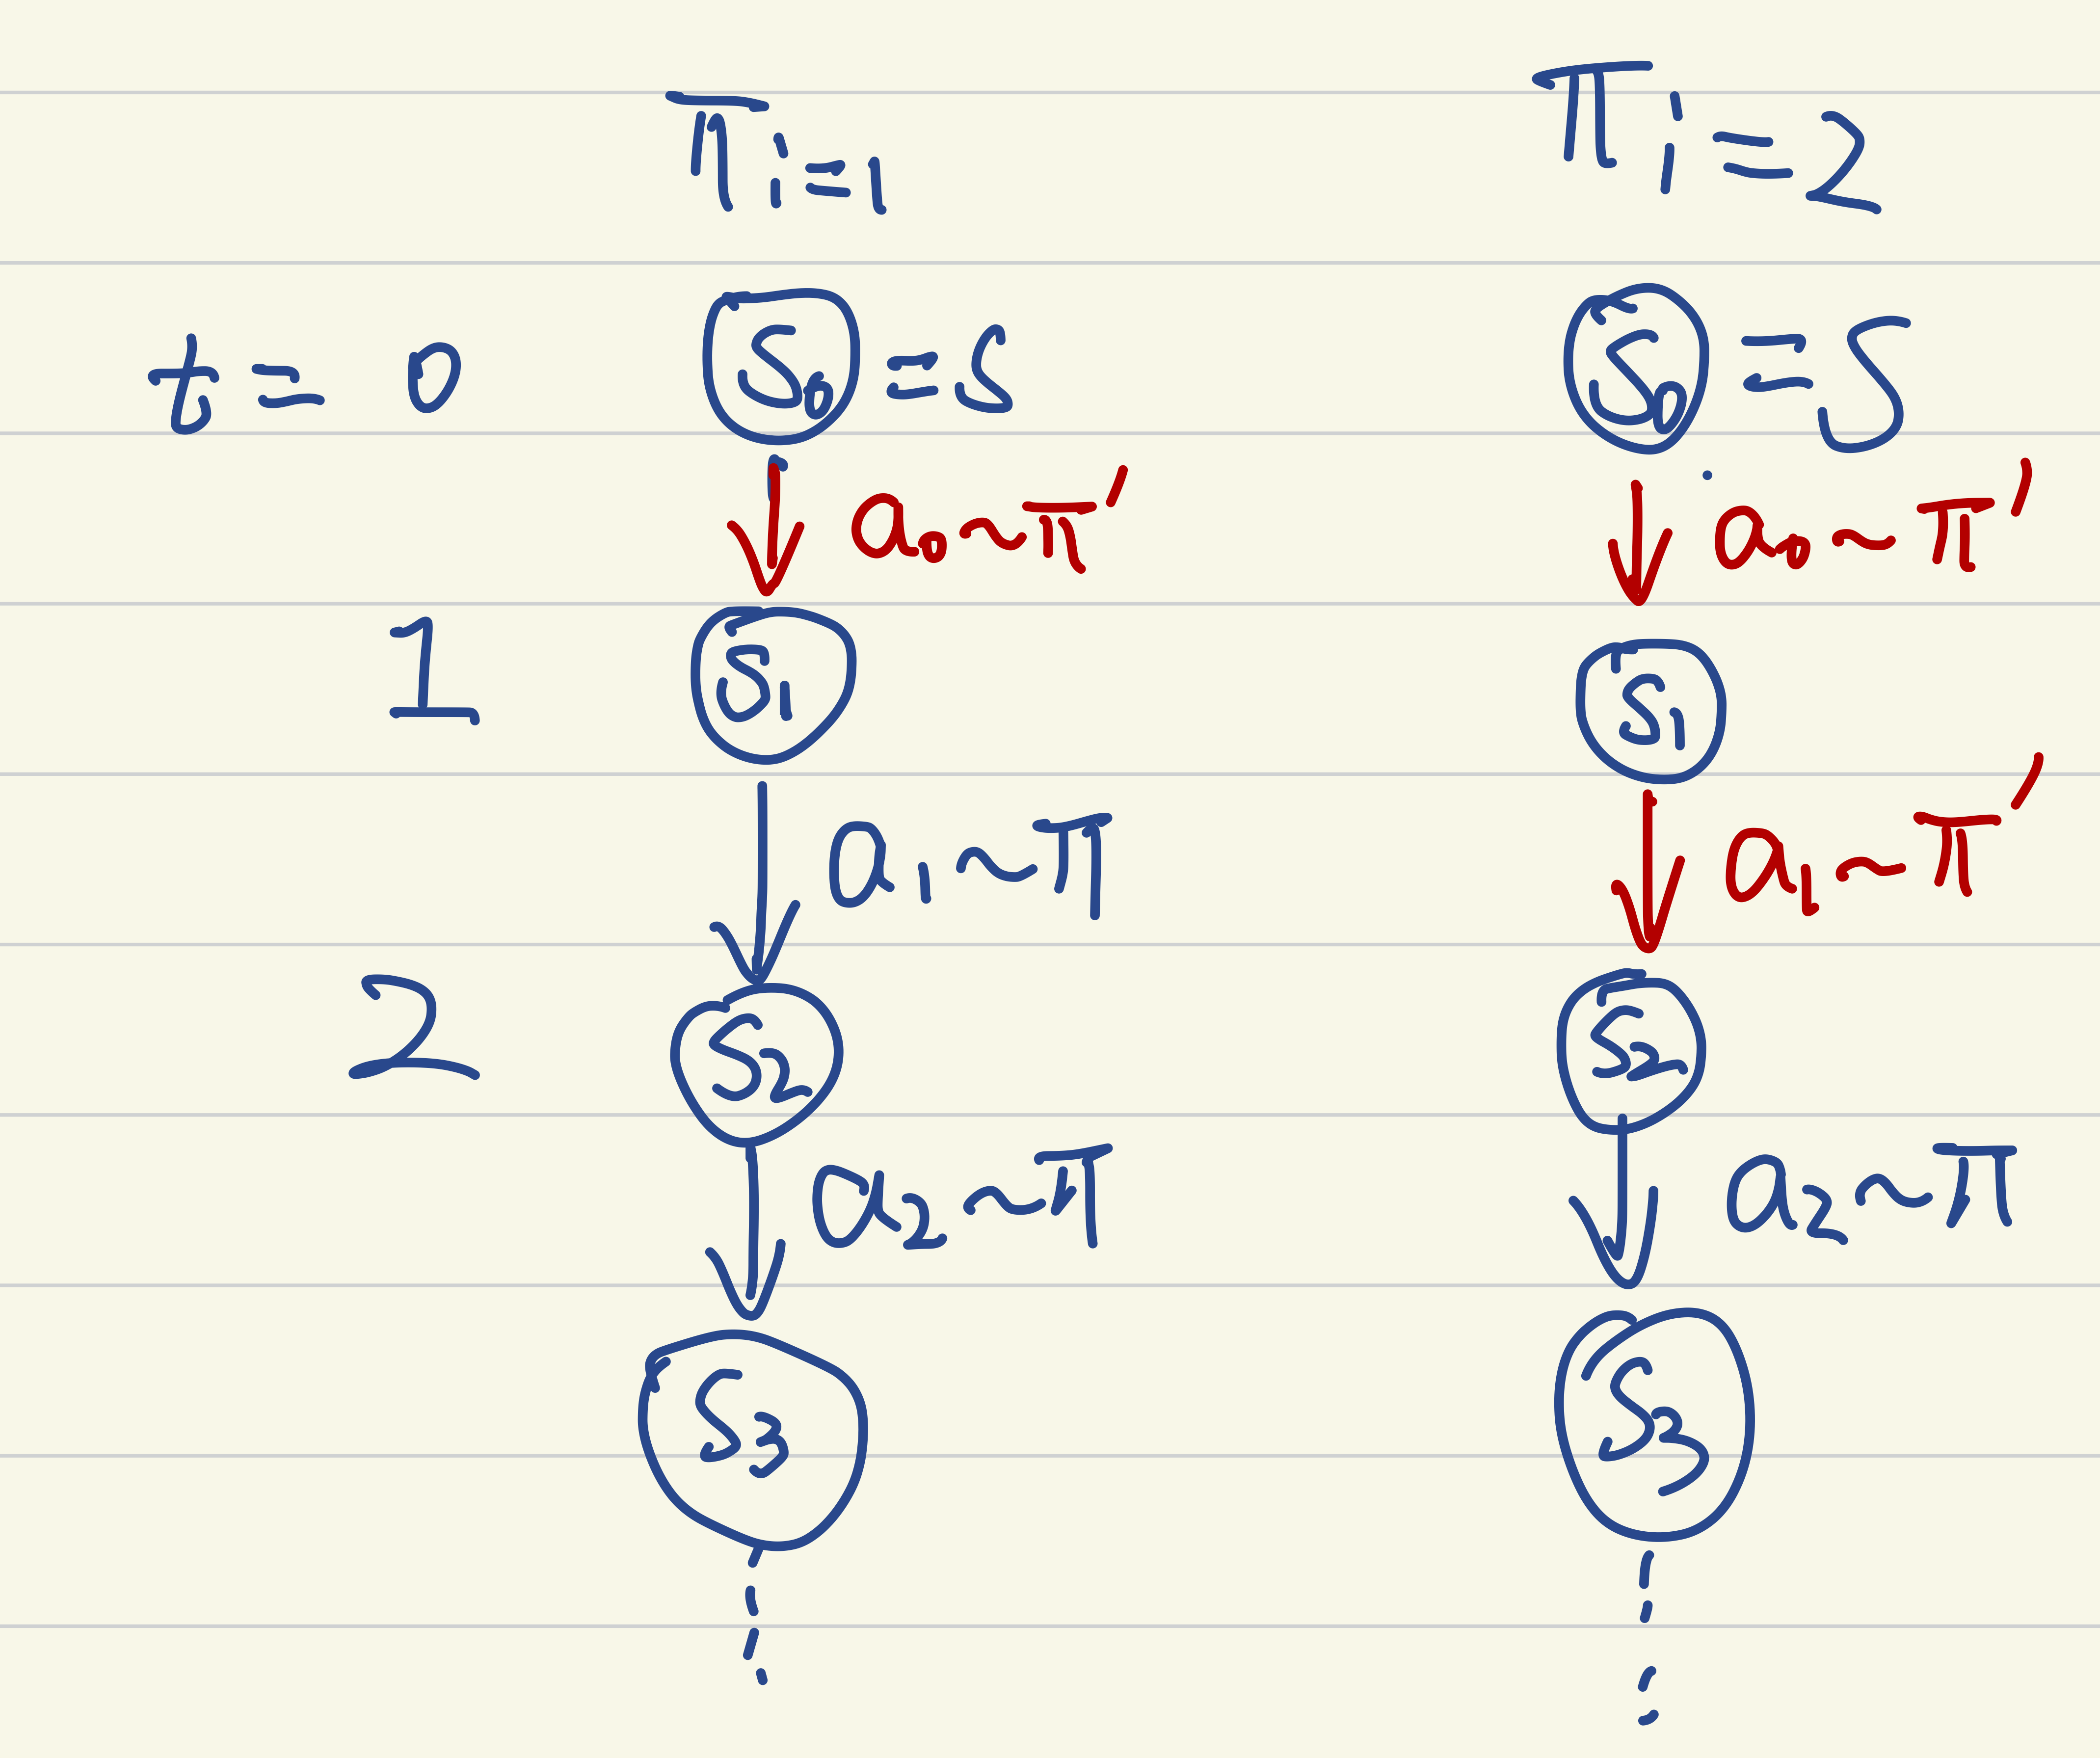
\includegraphics[scale=.7]{assignment1_2.png}
\centering
\end{figure}


Now we can rewrite the LHS of the statement as:
\begin{align*}
   V^{\pi'}(s) - V^{\pi}(s) = \sum_{i=0}^{\infty} (V^{\pi_{i+1}}(s) - V^{\pi_{i}}(s))
\end{align*}
For each term $(V^{\pi_{i+1}}(s) - V^{\pi_{i}}(s))$ on the RHS, observe that $\pi_{i+1}$ and  $\pi_{i}$ are both identical to $\pi'$ for the first $i$ time steps, which induces the same state distribution ate time step $i$, $\Pr(s_i|s_0=s, \pi')$.
They are also both identical to $\pi$ starting from state $s_{i+1}$ at time step $i+1$; so conditioned on $(s_i=s, a_i=a)$, the expected total reward for the remainder of the trajectory is $\gamma^i Q^\pi(s,a)$. Therefore, we have
\begin{align*}
    V^{\pi_{i+1}}(s) - V^{\pi_{i}}(s) = \gamma^i \sum_{s'}\Pr(s_i=s'|s_0=s, \pi')(\E_{a_i\sim \pi'(s')}[Q^\pi(s',a_i)]-\E_{a_i\sim \pi(s')}[Q^\pi(s',a_i)]).
\end{align*}
because the difference between $V^{\pi_{i+1}} - V^{\pi_{i}}$ only starts from $s_i$ at time step $i$, where $\pi_{i+1}$ and $\pi_{i}$ choose action $a_i$ according $\pi'$ and $\pi$, respectively.

\begin{shaded}
Your answer here.
\end{shaded}


\item Using the performance difference lemma, prove the policy improvement theorem, i.e. prove $V^{\pi_{k+1}}(s) \geq V^{\pi_{k}}(s)$, where $\pi_{k+1}$ and $\pi_{k}$ are consecutive policies in policy iteration.
\begin{shaded}
Your answer here.
\end{shaded}
\end{enumerate}



\newpage
\section{Bounding the Performance of Greedy Policy [25pt]}
\begin{enumerate}[label=(\alph*)]
    \item Consider the sequence of iterates, $V_0, V_1,...,V_k,...$, in value iteration, where $V_k = T^* V_{k-1}$.
    Suppose $\gamma<1$.
    Since $T^*$ is a contraction, $\norm{V_k-V_{k-1}}_\infty$ decreases as $k$ increases, $\norm{V_k-V_{k-1}}_\infty = \norm{T^*V_{k-1}-T^*V_{k-2}}_\infty \leq \gamma\norm{V_{k-1}-V_{k-2}}_\infty$.
    Suppose $\norm{V_k-V_{k-1}}_\infty \leq \epsilon$ for some large enough $k$.
    Show that $\norm{V^*-V_k}_\infty \leq \frac{\epsilon}{1-\gamma}$. In words, if the iterates are close, then they are close to the optimal state-value $V^*$.
    
    \underline{Hint:} Pick some integer $n\geq1$, we have 
    \begin{align*}
        \norm{V^*-V_k}_\infty =& \norm{V^*-V_{k+n} + V_{k+n} - V_{k+n-1} +...+V_{k+1}-V_k}_\infty \\
        \leq&  \norm{V^*-V_{k+n}}_\infty + \sum_{i=1}^{n} \norm{V_{k+i}-V_{k+i-1}}_\infty  \qquad \text {(triangle inequality)}
    \end{align*}
    \begin{shaded}
    Your answer here.
    \end{shaded}
    
    \item Suppose $\norm{V-V^*}_\infty\leq\epsilon$ for some $V\in\mathbb{R}^{|S|}$. Let $\pi$ be the greedy policy with respect to $V$, $\pi(s)=\argmax_a R(s,a) + \gamma  \sum_{s'}P(s'|s,a)V(s')$.
    Show that  $\norm{V^* -V^\pi}_\infty \leq \frac{2\gamma\epsilon}{1-\gamma}$.
    
    Hint: Using the fact that $T^\pi V = T^* V$ since $\pi$ is greedy with respect to $V$, write $\norm{V^* -V^\pi}_\infty = \norm{V^* -T^* V + T^\pi V - V^\pi}_\infty$ and apply the triangle inequality.
    \begin{shaded}
    Your answer here.
    \end{shaded}
\end{enumerate}


\newpage
\section{Frozen Lake MDP [25pt]}

Implement value iteration and policy iteration for the Frozen Lake environment
from \href{"https://gym.openai.com/envs/FrozenLake-v0"}{OpenAI Gym}. We have provided
custom versions of this environment in the starter code in folder \texttt{assignment1\_coding}.

Make sure you use Python 3 and have installed the dependencies in \texttt{requirements.txt}.

This problem is credited to Emma Brunskill.

\begin{enumerate}[label=(\alph*)]
\item \textbf{(coding)} Read through \texttt{vi\_and\_pi.py} and implement \texttt{policy\_evaluation}, \texttt{policy\_improvement} and \texttt{policy\_iteration}. The stopping tolerance (defined as $\max_s |V_{old}(s) - V_{new}(s)|$) is tol = $10^{-3}$. Use $\gamma = 0.9$. Return the optimal value function and the optimal policy.
\item \textbf{(coding)} Implement \texttt{value\_iteration} in \texttt{vi\_and\_pi.py}. The stopping tolerance is tol =
$10^{-3}$. Use $\gamma = 0.9$. Return the optimal value function and the optimal policy.
\item \textbf{(written)} Run both methods on the Deterministic-4x4-FrozenLake-v0 and Stochastic-4x4-FrozenLake-v0 environments. In the second environment, the dynamics of the world are stochastic. How does stochasticity affect the number of iterations required, and the resulting policy?
\begin{shaded}
    Your answer to (c) is here. For (a) and (b), submit the assignment1\_$\langle username \rangle$.zip file containing your implemented \texttt{vi\_and\_pi.py}.
\end{shaded}

\end{enumerate}


\end{document}